\section{Lecture 1: Introduction - 2 February 2026}
Outline:
\begin{enumerate}[label=(\Roman*)]
    \item Intro and Logistics
    \item Perspectives to Plans
    \item QM and Quantum Circuits
    \item Quantum Noise: Density Matrices
\end{enumerate}


\subsection{Lecture Perspective and Plan}
\begin{multicols}{2}
\textbf{Grading:}
\begin{enumerate}
  \item Homework: 15\%
  \item Participation: 10\%
  \item Project: 15\%
  \item Quizzes: 60\%
\end{enumerate}
\columnbreak
\textbf{Four units}
\begin{enumerate}
  \item Quantum Error Correction
  \item Quantum Algorithms
  \item Models of Fault Tolerant Quantum Computing
  \item Entanglement
\end{enumerate}
\end{multicols}
Goal: Be able to write research-quality papers\\
Schedule: 4 Modules - each with 1 quiz in class, 3 TPS (Think-Pair-Share)



\subsubsection{Quantum Error Correction (QEC)}
Encode: $a\ket{0} + b\ket{1} \mapsto a \ket{0_L} + b \ket{1_L}$ \\
What?: 
\begin{itemize}
    \item Method for reversing decoherence (quantum noise)
    \item Hiding from noise
    \item Controlling entropy
\end{itemize}
How?:
\begin{itemize}
    \item Embed our system into a larger system (embed into a larger Hilbert space)
    \item ``Church of the larger Hilbert space''
\end{itemize}
Why?:
\begin{itemize}
    \item In order to make quantum computing a reality, we have to deal with noise
    \item Security of Quantum Key Distribution
    \item Black Holes
\end{itemize}
Unknown?:
\begin{itemize}
    \item Efficiency: (how large of a system do we need to use to embed a small system in order to deal with the noise that we have) rates, overhead
    \item Given a code, is it locally testable? If so, we can prove the Probabilistically Checkable Proofs (PCP) theorem 
\end{itemize}



\subsubsection{Quantum Algorithms}
We can picture a quantum algorithm as something that takes in an input $x$ that encodes some kind of function and gives some output.  \\
\begin{center}
\begin{quantikz}
    & \gate[3]{U} & \\
    \lstick{$x$} & & \\
    & & 
\end{quantikz}
\end{center}
What?:
\begin{itemize}
    \item Mapping of problems onto quantum resources 
\end{itemize}
How?
Toffoli gate: output is Z XOR (X AND Y) This is universal for all reversible computation and all classical computation. Since this is a unitary gate
\begin{center}
    \begin{quantikz}
    \lstick{$x$} & \ctrl{2} & \\
    \lstick{$Y$} & \ctrl{1} & \\
    \lstick{$Z$} & \targ{} & \rstick{$Z \oplus XY$}\\
    \end{quantikz}
\end{center}

\begin{itemize}
    \item Reversible Quantum Computation
    \item Quantum Search
    \item Quantum Fourier Transform (QFT) $\rightarrow$ Factoring, Phase Estimation $HHL$ ($A\vec{x} = \vec{b}$)
    \item Quantum Simulation
    \item Grand unification of Quantum Algorithms: Quantum Singular Value Transform (Quantum signal processing)
\end{itemize}

Why?
\begin{itemize}
    \item Reveal the nature of mathematical problems (polynomial hierarchy)
    \item Nature of physical world (easy/hard)? 
    \item Practical applications (quantum computational sensing)
\end{itemize}

Unknowns?
\begin{itemize}
    \item When is quantum better than classical? (Quantum advantage)
    \item What is the hardness relative to noise? 
    \item what are hard/easy quantum transforms?
\end{itemize}

\subsubsection{Fault Tolerant Quantum Computing}
What?: 
\begin{quantikz}
    & \gate[3]{U} & \gate[3]{QEC} & \\
    \lstick{$x$} & & &\\
    & & &
\end{quantikz}
%\gategroup[3,steps=2,style={dashed,rounded corners}

What?:
\begin{itemize}
    \item Make reliable quantum systems from unreliable components (a human is an example)
\end{itemize}
How? 
\begin{itemize}
    \item von Neumann - compute on codes 
    \item Measurement induces change in the quantum systems $\rightarrow$ measurement-based computation
    \item Teleportation-based quantum computation
\end{itemize}
Why?
\begin{itemize}
    \item Useful quantum computation
    \item New physics?
    \item The transition between faulty $\leftrightarrow$ reliable is a phase transition; Fault tolerant threshold
\end{itemize}
Unknowns:
\begin{itemize}
    \item Fault tolerant threshold
    \item FTQC $\Leftrightarrow$ PICP (Probabilistically Checkable Proofs)
\end{itemize}



\subsubsection{Entanglement}
What?
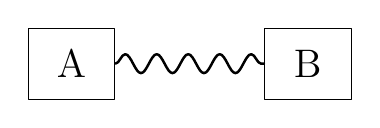
\begin{tikzpicture}[line cap=round, line join=round]

% Boxes
\node[draw, minimum width=1.1cm, minimum height=0.9cm] (A) at (0,0) {\Large A};
\node[draw, minimum width=1.1cm, minimum height=0.9cm] (B) at (3,0) {\Large B};

% Wavy connection
\draw[decorate, decoration={snake, amplitude=1.2mm, segment length=4mm}, line width=0.9pt]
  (A.east) -- (B.west);

\end{tikzpicture}
\begin{itemize}
    \item A new kind of physical resource
    \item Multi-party protocols
    \item Shared secret, communication
\end{itemize}
How?:
\begin{itemize}
    \item Non-local operators
    \item Communication bits $\rightarrow$ qubits
    \item Quantum measurement is akin to a one-way function
\end{itemize}
Why?:
\begin{itemize}
    \item No exponential quantum advantage without entanglement
    \item Provable exponential quantum communication advantage over classical 
    \item MIP$^{*}$ = RE, MIP = multiple provers, RE = recursively enumerable 
\end{itemize}
Unknowns?:
\begin{itemize}
    \item multi-partite entanglement
    \item entanglement + noise tends to destroy
\end{itemize}


\subsection{Quantum Mechanics and Quantum Circuits}
Four postulates:
\begin{itemize}
    \item State: system = unit vector $\ket{\psi}$ 
    \item Gate: $\ket{\psi'} = U \ket{\psi}$ 
    \item Measurement: $\{m_k\}$ s.t. $\sum_k m_k^\dagger m_k = I$ (completeness theorem); when measured $\ket{\psi}$ collapses $\ket{\psi} \mapsto \frac{m_k\ket{\psi}}{\sqrt{p_k}}$, where $p_k = \braket{\psi|m_k^\dagger m_k|\psi}$
    \item Composition: Tensor (Kronecker) Product 
\end{itemize}
Quantum Circuits:
\begin{itemize}
    \item Qubit 
        \begin{quantikz}
            & \qwbundle{} & 
        \end{quantikz}
    \item Bit
        \begin{quantikz}
            & \setwiretype{c} & 
        \end{quantikz}
    \item Gates
        \begin{quantikz}
            & \gate{U} & 
        \end{quantikz}
    \item Entangled States
        \begin{quantikz}
            \makeebit{} & & \\
            & &
        \end{quantikz}
\end{itemize}
Solovay-Kitaev Theorem: tells us how difficult it is to construct a given unitary gate $U$. The difficulty can be quantified. The quantification depends on the set of gates to construct. For a single qubit, we can construct any $U$ from $H,T$ \\
Solovay-Kitaev: any single qubit gate can be described by a string of $H$ and $T$ gates ( with each addition gate doubles the precision, $H$ and $T$ are like binary matrix digits) \\  
\begin{quantikz} & \gate{U} &\end{quantikz} $\doteq$ \begin{quantikz} & \gate{H} &\end{quantikz} $H = \frac{1}{\sqrt{2}}\begin{pmatrix}1 & 1 \\ 1 & -1\end{pmatrix}$, \\
\hspace*{2.3cm}\begin{quantikz} & \gate{S} &\end{quantikz} $ S = \sqrt{Z} = \frac{1}{\sqrt{2}}\begin{pmatrix}1 & 0 \\ 0 & i\end{pmatrix}$\\
\hspace*{2.3cm}\begin{quantikz} & \gate{T} &\end{quantikz} $ T = \sqrt{S} = \frac{1}{\sqrt{2}}\begin{pmatrix}1 & 0 \\ 0 & e^{i\frac{\pi}{4}}\end{pmatrix} \leftarrow \frac{\pi}{8}$ gate  \\
$H, T$ and $CNOT$ gives us all universal


\subsection{Quantum Noise and Density Matrices}
Motivation Question: Given $\ket{\psi}$ or $\phi$ with probability $\frac{1}{2}$. What state? $\rho = \frac{1}{2}\ketbra{\psi}{\psi} + \frac{1}{2} \ketbra{\phi}{\phi}$ 

\begin{definition}
    A matrix $\rho$ is a density matrix iff a) $\Tr \rho = 1$, b) $\rho \geq 0$ i.e. $\forall \ket{\phi}$, $\braket{\phi|\rho|\phi} \geq 0$ and real ($\rho$ is positive definite and Hermitian)
\end{definition}

\begin{claim}
    $\rho = \sum p_k \ketbra{\psi_k}$, where $p_k$ are probabilities and sum to 1, is a legal density matrix. \\
     $\Tr \rho = 1$ and $\braket{\phi|\rho|\phi} = p_k \braket{\phi|\psi_k} \braket{\psi_k|\phi}$
\end{claim} 

\begin{claim}
    Any $\rho$ can be expressed as $\rho = \sum_k p_k \ketbra{\psi_k}{\psi_k}$ where $\sum_k p_k = 1$. (Proof by spectral decomposition: $p_k$ are eigenvalues and $\ket{\psi}$ are eigenvectors)
\end{claim}

\begin{definition}
    A density matrix $\rho$ is pure iff $\rho = \ketbra{\psi}$
\end{definition}

\begin{example}
    Is $\rho = p_k \rho_k$ a legal density matrix? Yes\\
    Is $\rho = \frac{1}{2}\begin{pmatrix}1 & 0 & 0 & 0 \\ 0 & 0 & 1 & 0 \\ 0 & 1 & 0 & 0 \\ 0 & 0 & 0 & 1 \end{pmatrix}$ a legal density matrix? No, because the block in the middle is the $X$ matrix $\begin{pmatrix}0 & 1 \\ 1 & 0 \end{pmatrix}$, which have eigenvalues $\pm 1$.  
\end{example}

\begin{lemma}
    von Neumann unravellings: \\
    Let $\rho = \sum p_k \ketbra{\psi_k}$. Then $\rho = \rho' = \sum_i q_i \ketbra{\phi_i}$, where $\ket{\psi}$  and $\ket{\phi}$ iff $\sqrt{p_k} \ket{\psi_k} =  \sum_j U_{kj} \ket{\phi_j}$
\end{lemma}
If a density matrix is not legal, it cannot describe a physical system. Otherwise, any density matrix can be physically realized if it is a legitimate density matrix. (1-1 with physical reality) 

\begin{example}
    Suppose $\rho = \frac{1}{2} \begin{pmatrix}1 & 0 \\ 0 & 1\end{pmatrix} = \frac{1}{2} \ketbra{0} + \frac{1}{2} \ketbra{1} = \frac{1}{2} \ketbra{+} + \frac{1}{2} \ketbra{-}$     
\end{example}
Avoid preferred ensemble fallacy!